\documentclass[tikz]{standalone}
\usepackage{float}              % [H]
\usepackage{graphicx}           % (pdf, png, jpg, eps)
\usepackage{pgfplots}
\usepackage{siunitx}
\usepackage{currfile}
\usepackage{ifthen}
\usepackage{tikz}
\usepackage{mathtools}
\usetikzlibrary{calc}
\usepackage{pgfplots}
\usepackage{pgfplotstable}
\pgfplotsset{compat=1.17}
\usepgfplotslibrary{colorbrewer}
\usepgfplotslibrary{groupplots}
\usepgfplotslibrary{statistics}
% \usetikzlibrary{external}
% \tikzexternalize
\tikzset{>=latex}
\DeclarePairedDelimiter\abs{\lvert}{\rvert}
\DeclareSIUnit{\arbitraryunit}{a.u.}
% 
\def\width{13.87303cm}
\def\height{22.37076cm}
\def\datapath{../../__PATH__}
\directlua0{
  pdf.setinfo ("/Path: (__PATH__)")
}
% 
\begin{document}
\pgfmathsetmacro{\ng}{5}
\pgfmathsetmacro{\dx}{0.65}
% 
\pgfplotsset{colormap/Paired-5}
\pgfplotsset{
    Boxplot/.style={
        cycle list/Paired-5,
        boxplot={
            draw position={1-\dx/2+floor((\plotnumofactualtype+0.001)/\ng) + \dx/(\ng-1)*mod(\plotnumofactualtype,\ng)},
            box extend=\dx/(\ng+1),
            mark size=0.1pt,
            mark options={fill=black},
            draw/median/.code={%
               \draw[mark size=2pt,/pgfplots/boxplot/every median/.try]
               \pgfextra
               \pgftransformshift{
                  \pgfplotsboxplotpointabbox
                     {\pgfplotsboxplotvalue{median}}
                     {0.5}
               }
               \pgfuseplotmark{*}
               \endpgfextra
               ;
            },
        },
        boxplot/draw direction=y,
    },
} 
%
\foreach \setup [count=\k] in {PM} { % LAP
\foreach \species [count=\l] in {Roden,Vervet,Human} { % {Roden,Vervet,Human}
% 
\begin{tikzpicture}[]
\begin{axis}[%
   width = 0.1*\width,
   height = 0.22*\height,
   scale only axis,
   xmin=0.42,
   xmax=1.58,
   axis x line=none,
   axis y line=left,
   enlarge y limits,
   ymajorgrids,
   clip=false,
   ylabel={transmittance / $\si{\arbitraryunit}$},
   ylabel absolute, every axis y label/.append style={yshift=0.0ex},
   Boxplot,
   ]
\foreach \dn [count=\idn] in {0.008}{ %0.002,0.004,0.006,0.008,0.01
   \foreach \r in {0.5,1.0,2.0,5.0,10.0}{
      \addplot+[fill, draw=black] table[%
         y={\r_\dn}, col sep=comma, row sep=newline,
         ]{\datapath/transmittance_\setup_\species.csv};
   }
}
\draw[decorate,decoration={brace,amplitude=1ex,mirror},white]
   ({axis cs:0.6,0.0} |- {axis description cs:0.0,0.0}) --
   ({axis cs:1.4,0.0} |- {axis description cs:0.0,0.0})
   node [white,midway,below,yshift=-1ex, align=left]
   {\footnotesize \phantom{$\Delta n = \SI{0.002}{}$}};
\end{axis}
\end{tikzpicture}
}}
% 
\foreach \setup [count=\k] in {PM} { % LAP
\foreach \species [count=\l] in {Roden,Vervet,Human} { % {Roden,Vervet,Human}
% 
\begin{tikzpicture}[]
\begin{axis}[%
   width = 0.6*\width,
   height = 0.22*\height,
   scale only axis,
   xmin=0.42,
   xmax=5.58,
   axis x line=none,
   axis y line=left,
   enlarge y limits,
   ymajorgrids,
   clip=false,
   ylabel={retardation},
   ylabel absolute, every axis y label/.append style={yshift=0.0ex},
   Boxplot,
   ]
\foreach \dn [count=\idn] in {0.002,0.004,0.006,0.008,0.01}{
   \foreach \r in {0.5,1.0,2.0,5.0,10.0}{
      \addplot+[fill, draw=black] table[%
         y={\r_\dn}, col sep=comma, row sep=newline,
         ]{\datapath/retardation_\setup_\species.csv};
   }
}
\draw[decorate,decoration={brace,amplitude=1ex,mirror}]
   ({axis cs:0.6,0.0} |- {axis description cs:0.0,0.0}) --
   ({axis cs:1.4,0.0} |- {axis description cs:0.0,0.0})
   node [black,midway,below,yshift=-1ex, align=left]
   {\footnotesize $\Delta n = \SI{0.002}{}$};
\draw[decorate,decoration={brace,amplitude=1ex,mirror}]
   ({axis cs:1.6,0.0} |- {axis description cs:0.0,0.0}) --
   ({axis cs:2.4,0.0} |- {axis description cs:0.0,0.0})
   node [black,midway,below,yshift=-1ex, align=left]
   {\footnotesize $\Delta n = \SI{0.004}{}$};
\draw[decorate,decoration={brace,amplitude=1ex,mirror}]
   ({axis cs:2.6,0.0} |- {axis description cs:0.0,0.0}) --
   ({axis cs:3.4,0.0} |- {axis description cs:0.0,0.0})
   node [black,midway,below,yshift=-1ex, align=left]
   {\footnotesize $\Delta n = \SI{0.006}{}$};
\draw[decorate,decoration={brace,amplitude=1ex,mirror}]
   ({axis cs:3.6,0.0} |- {axis description cs:0.0,0.0}) --
   ({axis cs:4.4,0.0} |- {axis description cs:0.0,0.0})
   node [black,midway,below,yshift=-1ex, align=left]
   {\footnotesize $\Delta n = \SI{0.008}{}$};
\draw[decorate,decoration={brace,amplitude=1ex,mirror}]
   ({axis cs:4.6,0.0} |- {axis description cs:0.0,0.0}) --
   ({axis cs:5.4,0.0} |- {axis description cs:0.0,0.0})
   node [black,midway,below,yshift=-1ex, align=left]
   {\footnotesize $\Delta n = \SI{0.01}{}$};
% 
\end{axis}
\end{tikzpicture}
}}
% 

% LEGENDE
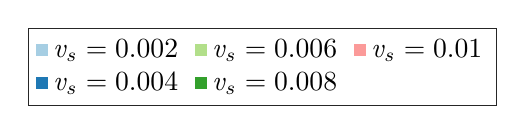
\begin{tikzpicture}[] 
\begin{axis}[%
    hide axis,
    scale only axis,
    height=0pt,
    width=0pt,
    cycle list/Paired-5,
    legend style={draw=white!15!black,legend cell align=left},
    legend transposed=true,
    legend columns=2,
    legend style={/tikz/every even column/.append style={column sep=1ex}},
    legend entries={%
        {$\mathit{v_{s}}=\SI{0.002}{}$},
        {$\mathit{v_{s}}=\SI{0.004}{}$},
        {$\mathit{v_{s}}=\SI{0.006}{}$},
        {$\mathit{v_{s}}=\SI{0.008}{}$},
        {$\mathit{v_{s}}=\SI{0.01}{}$},
    },
    legend image post style={mark=square*, only marks},
    ]
    \addplot+[] coordinates {(0,0)};
    \addplot+[] coordinates {(0,0)};
    \addplot+[] coordinates {(0,0)};
    \addplot+[] coordinates {(0,0)};
    \addplot+[] coordinates {(0,0)};
\end{axis} 
\end{tikzpicture}
% 
\end{document}
